\documentclass[a4paper,12pt,french]{book}
\usepackage[margin=2cm]{geometry}
\usepackage[thinfonts]{uglix2}
\nouveaustyle

\begin{document}
\titre{Processus TP3}{NSI2}{2021} 

Pour signifier qu'un processus \textbf{attend d'acquérir} une ressource, on dessine ceci :
\begin{center}
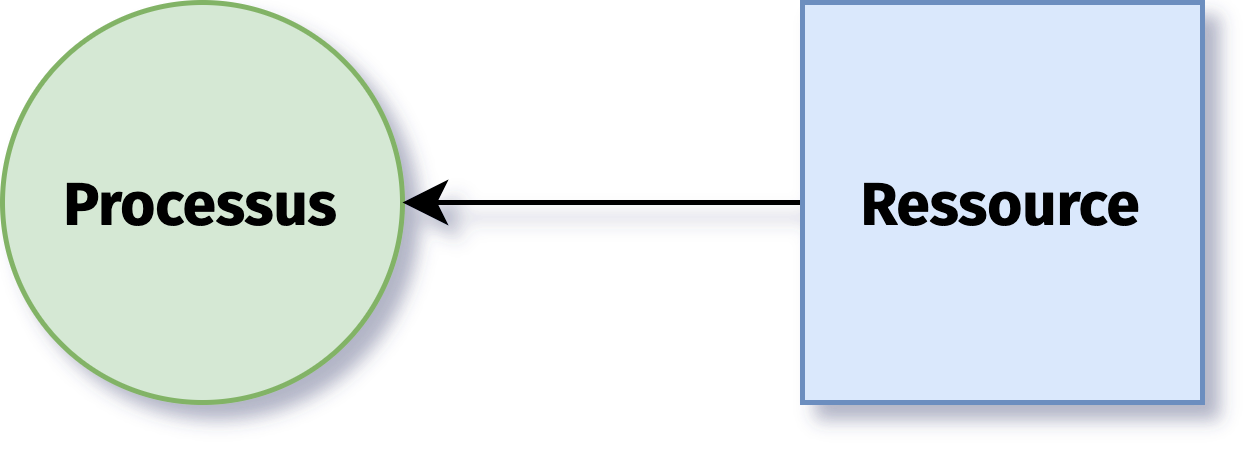
\includegraphics[width=4cm]{img/d1}
\end{center}

Pour signifier qu'un processus \textbf{détient} d'une ressource, on dessine ceci :
\begin{center}
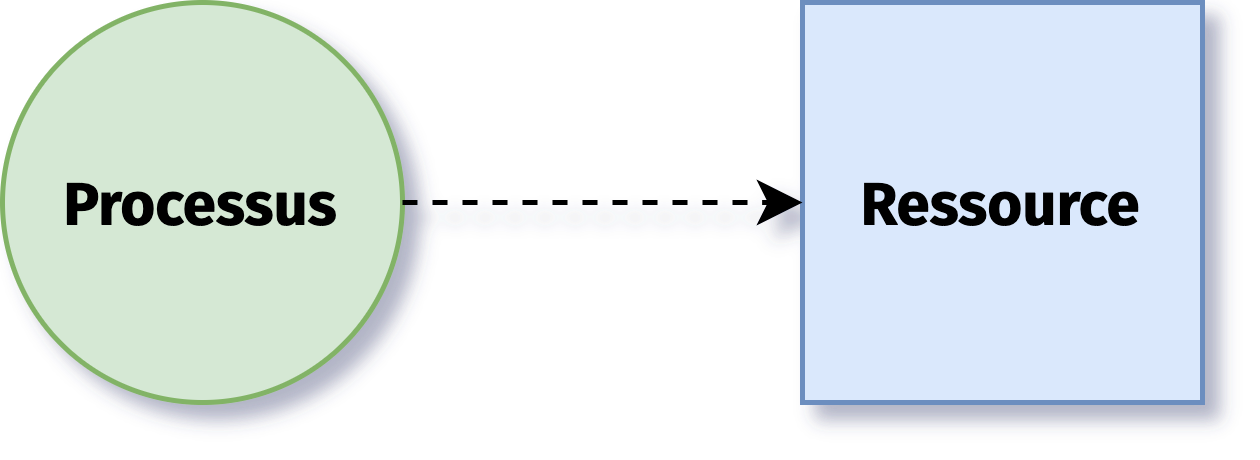
\includegraphics[width=4cm]{img/d2}
\end{center}

À chaque instant d'un scénario donné comportant des processus et des ressources, on peut donc dessiner le \textbf{graphe d'allocation des ressources}.
Une situation d'\textbf{interblocage} survient si, à un instant donné, le graphe comporte un \textbf{circuit} (suite d'arcs consécutifs dont les deux sommets extrémités sont identiques), tel l'exemple suivant :

\begin{center}
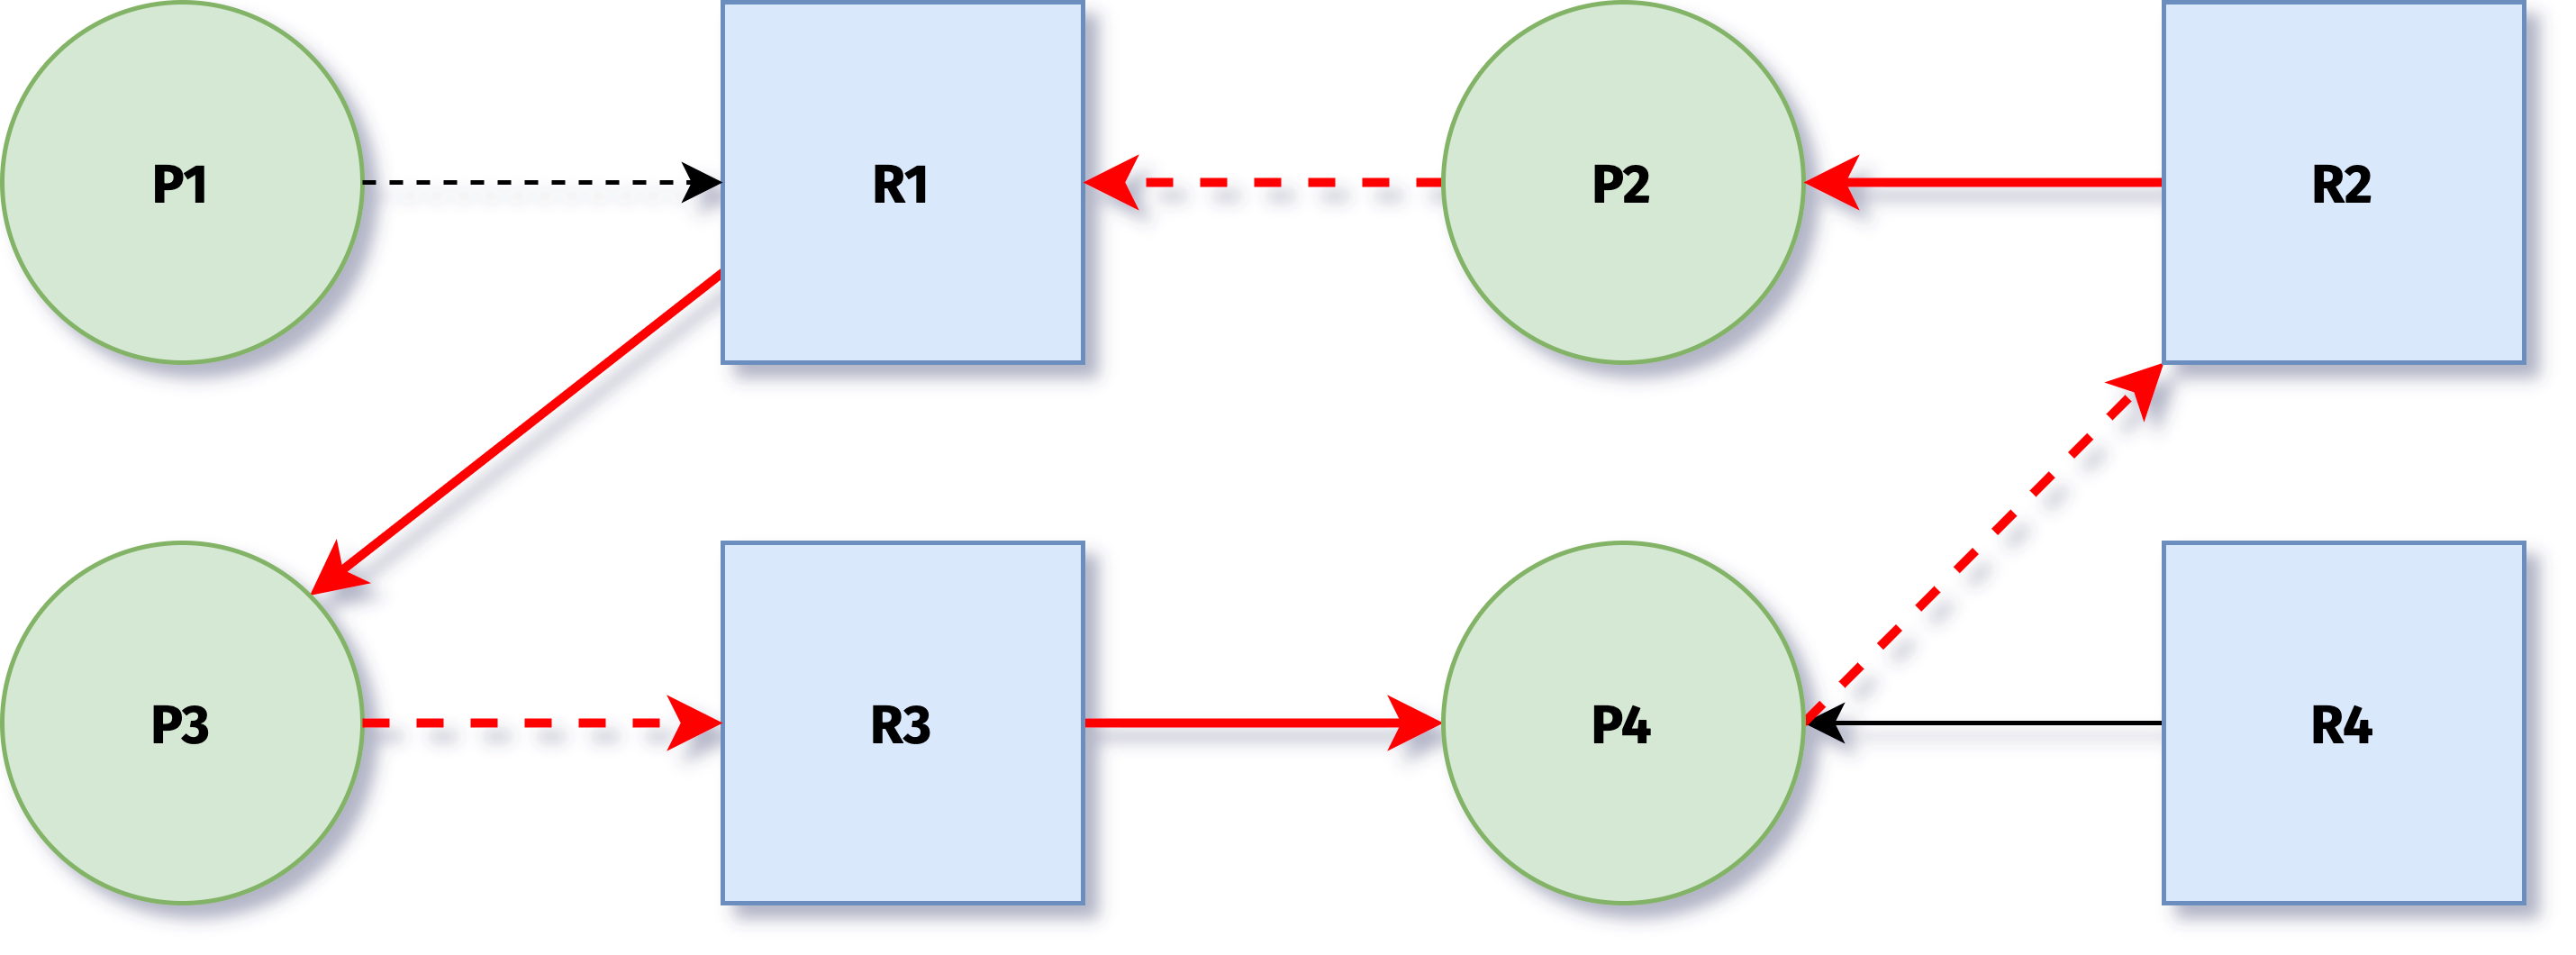
\includegraphics[width=9cm]{img/d5}
\end{center}
Le circuit R1-P3-R3-P4-R2-P2-R1 montre le phénomène d'\textbf{attente circulaire}.

\begin{exercice}[]
Y a-t-il interblocage ? Si oui préciser le circuit.
\begin{center}
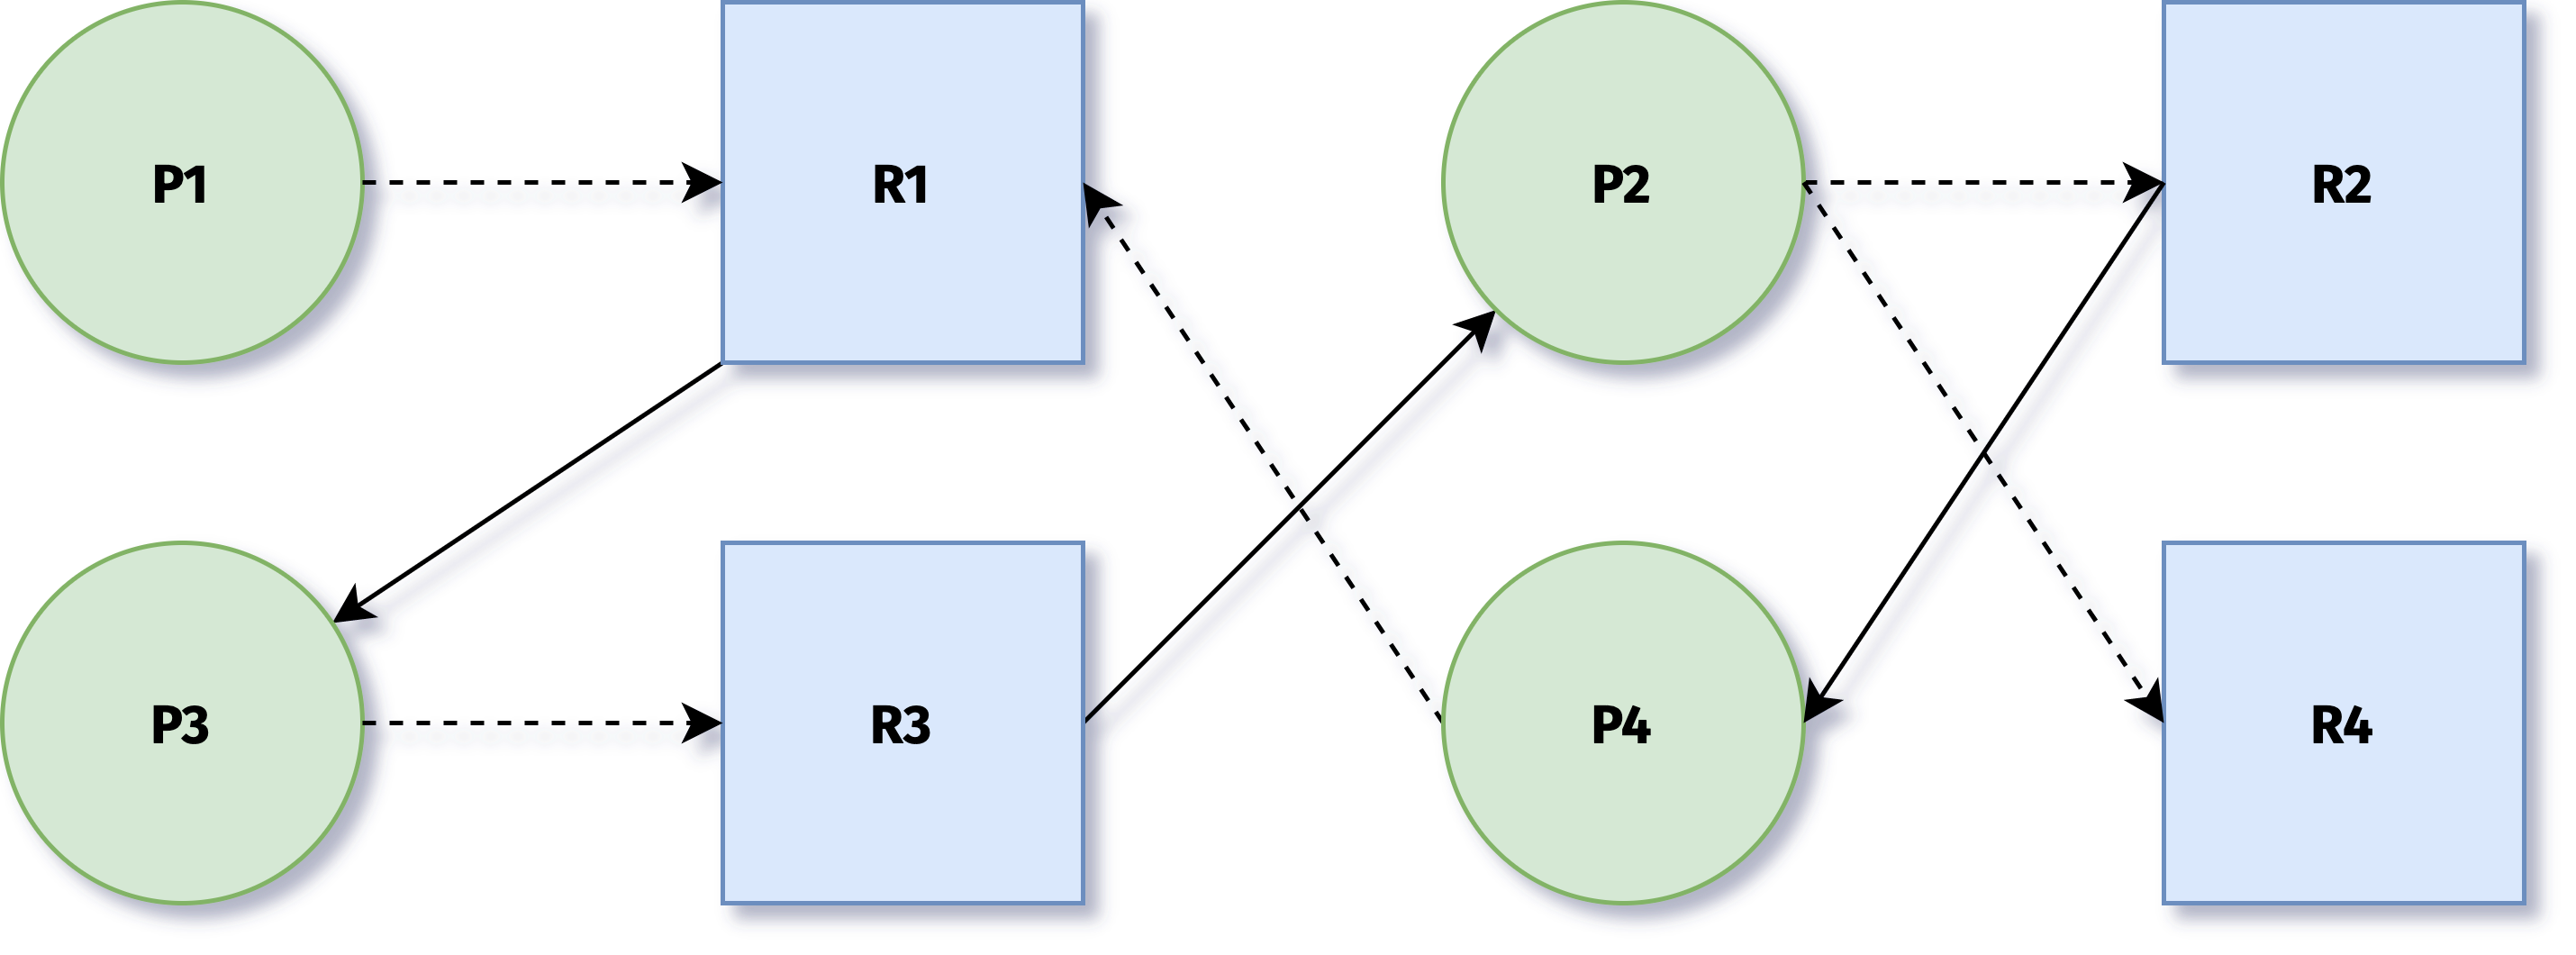
\includegraphics[width=9cm]{img/d3}
\end{center}
\end{exercice}

\begin{exercice}[]
Y a-t-il interblocage ? Si oui préciser le circuit.
\begin{center}
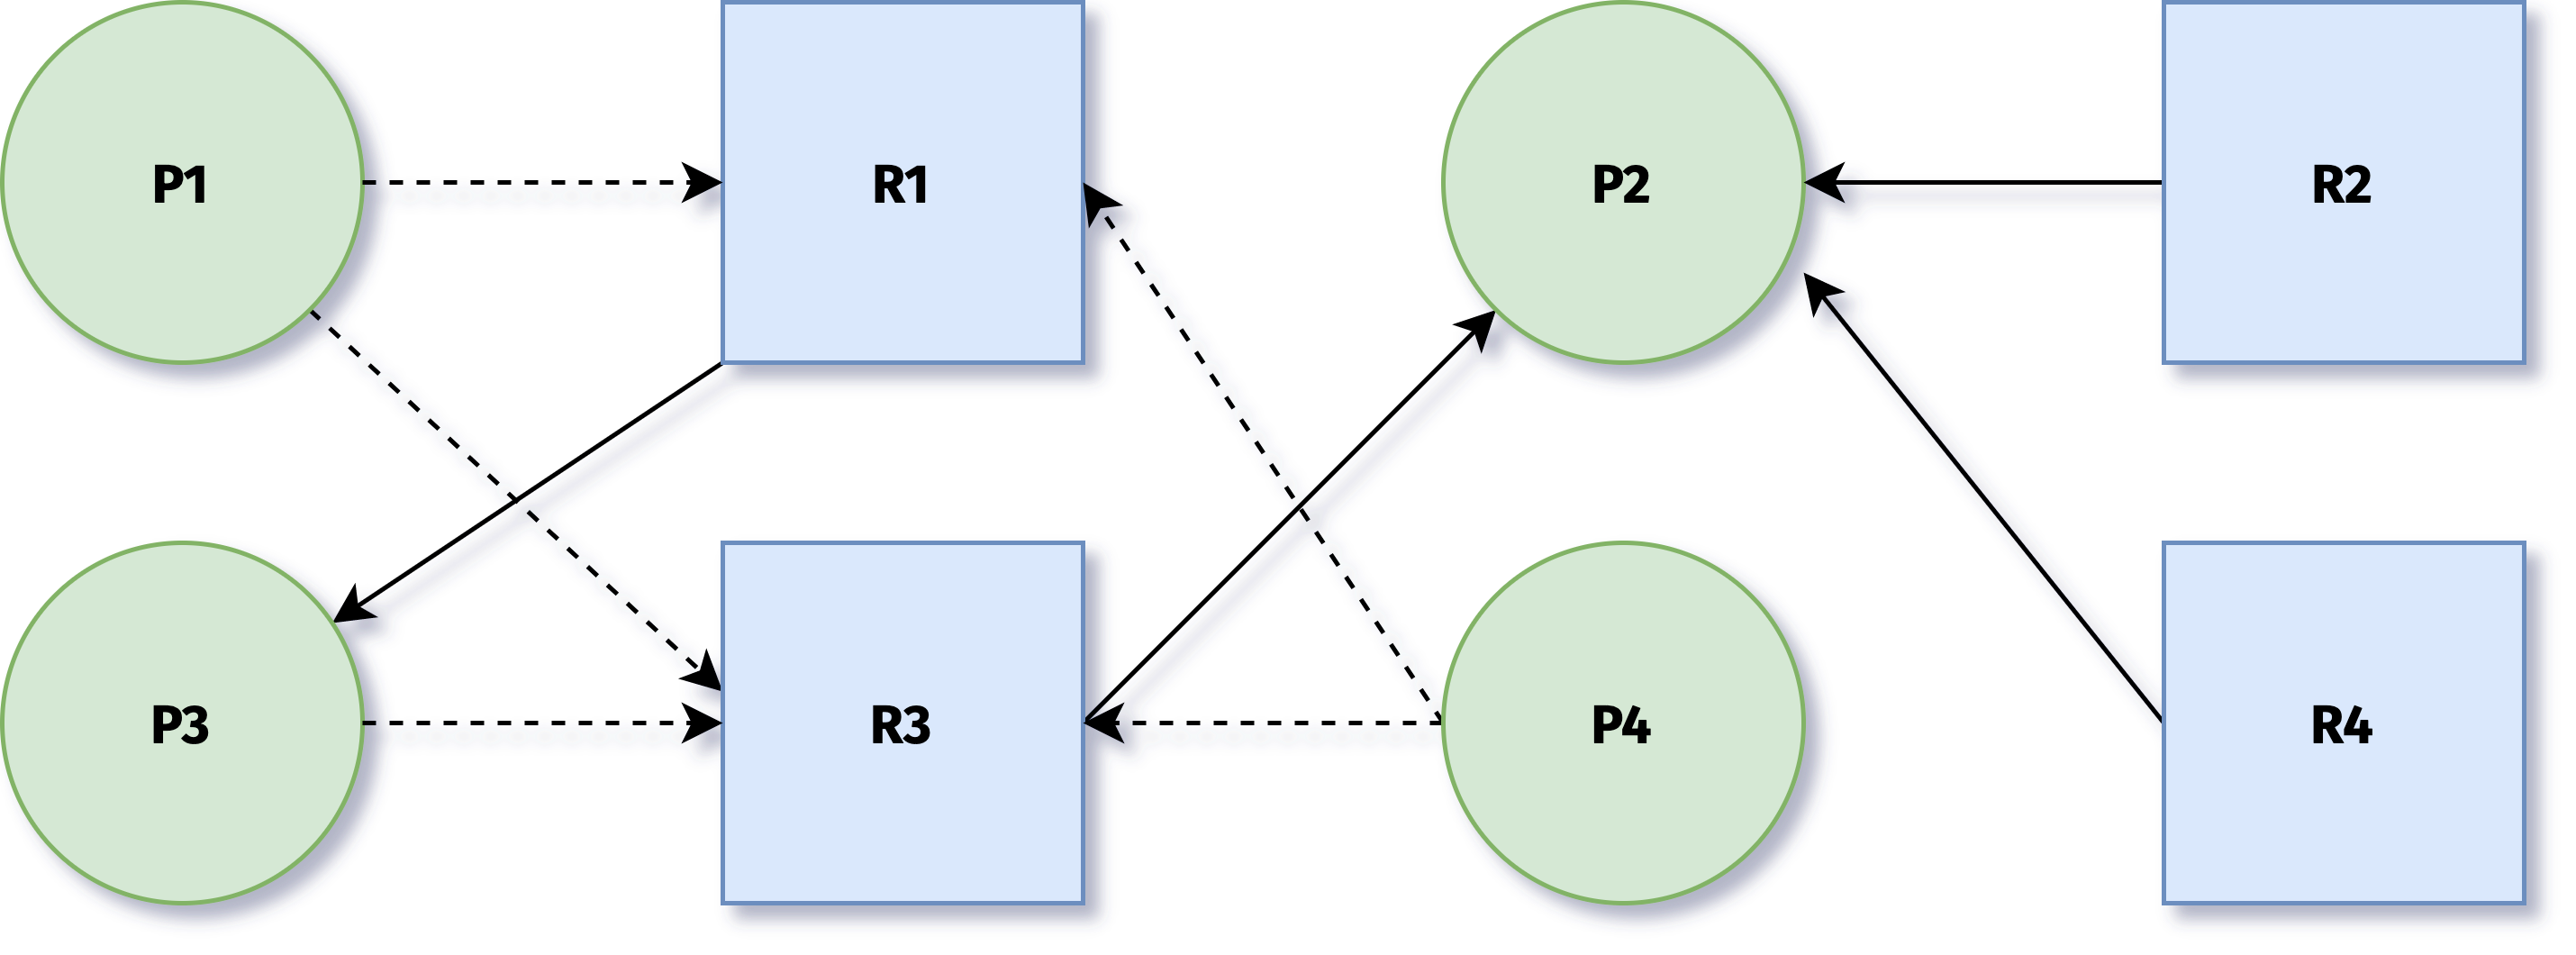
\includegraphics[width=9cm]{img/d4}
\end{center}
\end{exercice}
\begin{exercice}[]
Tracer le graphe d’allocation des ressources correspondant :
\begin{center}
\begin{tabular}{|c|c|c|}
\hline
\rowcolor{UGLiOrange} \textbf{\color{white}Processus }& \textbf{\color{white}Ressources demandées} & \textbf{\color{white}Ressources détenues} \\
\hline
A & 2 & 1 \\
\hline
B & 3 &  \\
\hline
C & 2 &  \\
\hline
D & 2 et 3 & 4 \\
\hline
E & 5 & 3 \\
\hline
F & 2 & 6 \\
\hline
G & 4 & 5 \\
\hline
\end{tabular}
\end{center}
Y a-t-il interblocage ? Si oui, préciser le cycle.
\end{exercice}
\begin{exercice}[]
On considère 3 processus P1, P2, P3 et 3 ressources R1, R2 et R3.\\
En traçant étape par étape le graphe d'allocation des ressources, expliquer pourquoi il y a interblocage.

\begin{enumerate}[\bfseries 1.]
	\item 	P2 demande R1
    \item 	P3 demande R2
    \item 	P1 demande R1
    \item 	P3 demande R3
    \item 	P2 libère R1
    \item 	P1 demande R2
    \item 	P3 demande R1  
\end{enumerate}
\end{exercice}

\begin{exercice}[]
On considère un robot pilotable à distance qui effectue en parallèle les processus suivants :
\begin{enumerate}[--]
	\item 	\textbf{P1  Pilotage manuel : } reçoit ordres via wifi et active moteurs en conséquence
	\item 	\textbf{P2  Envoi flux vidéo : } envoi du flux vidéo de la caméra via la liaison wifi
    \item 	\textbf{P3  Auto-test matériel : } tests des composants embarqués (hors communication réseau)
\end{enumerate}
Il dispose des ressources suivantes :
\begin{enumerate}[--]
	\item 	\textbf{R1 : }  moteurs
	\item 	\textbf{R2 : }  wifi
    \item 	\textbf{R3 : }	caméra
\end{enumerate}
Voici ce qui doit être exécuté (on n'indique pas les étapes de traitement des données):

\begin{center}
\begin{tabular}{|c|c|c|}
\hline
\rowcolor{UGLiOrange} \textbf{\color{white}P1 }& \textbf{\color{white}P2} & \textbf{\color{white}P3} \\
\hline
demande \textbf{R1} (moteurs) & demande \textbf{R2} (wifi) & demande \textbf{R3} (caméra) \\
\hline
demande \textbf{R2} (wifi) & demande \textbf{R3} (caméra) &  demande \textbf{R1} (moteurs) \\
\hline
libère \textbf{R1} (moteurs) & libère \textbf{R2} wifi & libère \textbf{R3} (caméra)  \\
\hline
libère \textbf{R2} (wifi) & libère \textbf{R3} caméra & libère \textbf{R1} (moteurs)  \\
\hline
\end{tabular}
\end{center}
On admet que l'ordonnanceur de l'OS exécute un seul processus à la fois et que les ressources sont à usage exclusif.
\begin{enumerate}[\bfseries 1.]
	\item 	Montrer que si l'ordonnancement commence par  P1 P3 P1 P3 P2 P1 alors il n'y a pas d'interblocage
	\item 	Trouver un scénario d'ordonnancement qui conduit à un interblocage.
\end{enumerate}
\end{exercice}

\end{document}